This thesis project has involved the implementation and evaluation
of many different components to create an end-to-end wheelchair
navigation assistance system.

\subsection{Evaluation of machine learning models on preliminary dataset}
%include speed 

\subsection{Transfer learning on Hybridnets model to improve performance}
% do this first
In the last section, it was seen that the Hybridnets model generalised well in most cases,
however struggled with some non-uniform pathways such as paved brick.
The model was originally trained on the BDD100K dataset, which 

\pagebreak
\subsection{Identification of suitable driving paths using segmentation}
% transformation, morphology, depth modes
The output of the Hybridnets drivable area segmentation model is a
segmentation mask, an array that indicates which pixels are drivable
and which are not.
This output must be transformed into a 2D birds-eye view occupancy map,
which indicates the drivable area around the wheelchair. This birds-eye
view occupancy map is a simplified representation of the surrounding world,
and is used as an input to the wheelchair control algorithms.

The ZED Mini 3D point cloud data was used
to transform the segmentation mask into an occupancy grid.
The ZED SDK uses the pinhole camera model, as seen in \cref{fig:pinhole_camera_model},
to describe the relationship between pixels on the image plane
and the coordinates of corresponding objects.
The point cloud data is represented as an array the same size as
the original image, with each pixel containing XYZ data about the location of that object
in 3D space.
% add representation diagram
\begin{figure}[b]
    \centering
    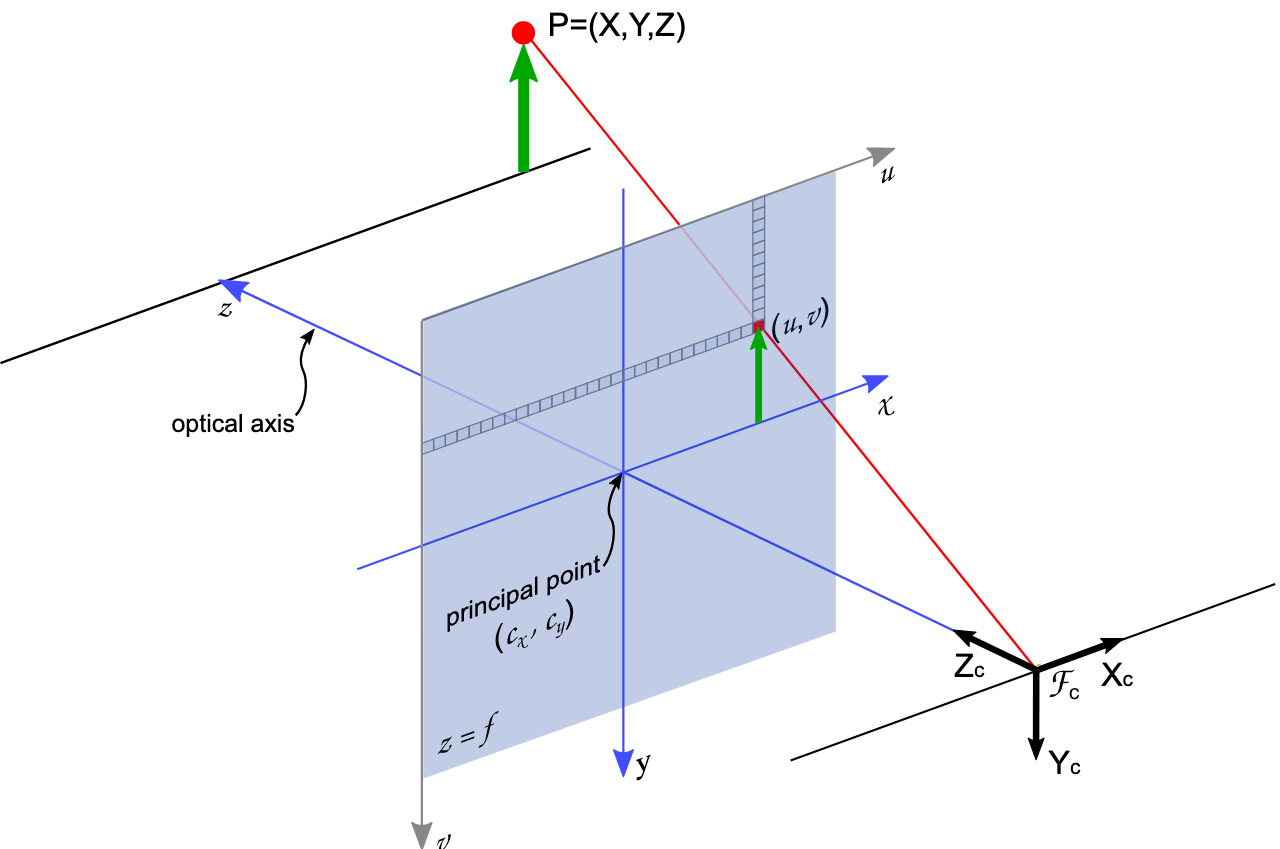
\includegraphics[width=0.6\linewidth]{images/pinhole_camera_model.png}
    \caption{Pinhole camera model. Reproduced from Nvidia \cite{nvidiaVisionProgrammingInterface}}
    \label{fig:pinhole_camera_model}
\end{figure}

To obtain the occupancy map, the point cloud is first filtered using the segmentation mask so that
non-drivable points are removed. The ZED SDK is unable to resolve the depth of some pixels
and instead represents their location as \texttt{nan}; these points are also removed.
Next, the array is simplified by removing non-essential information such as colour and altitude
data. What remains is an array of XZ points that represent drivable areas
identified by the segmentation algorithm. A right-handed y-up coordinate frame
was used (\cref{fig:zed_mini_coordinate_frame}).
\begin{figure}[b]
    \centering
    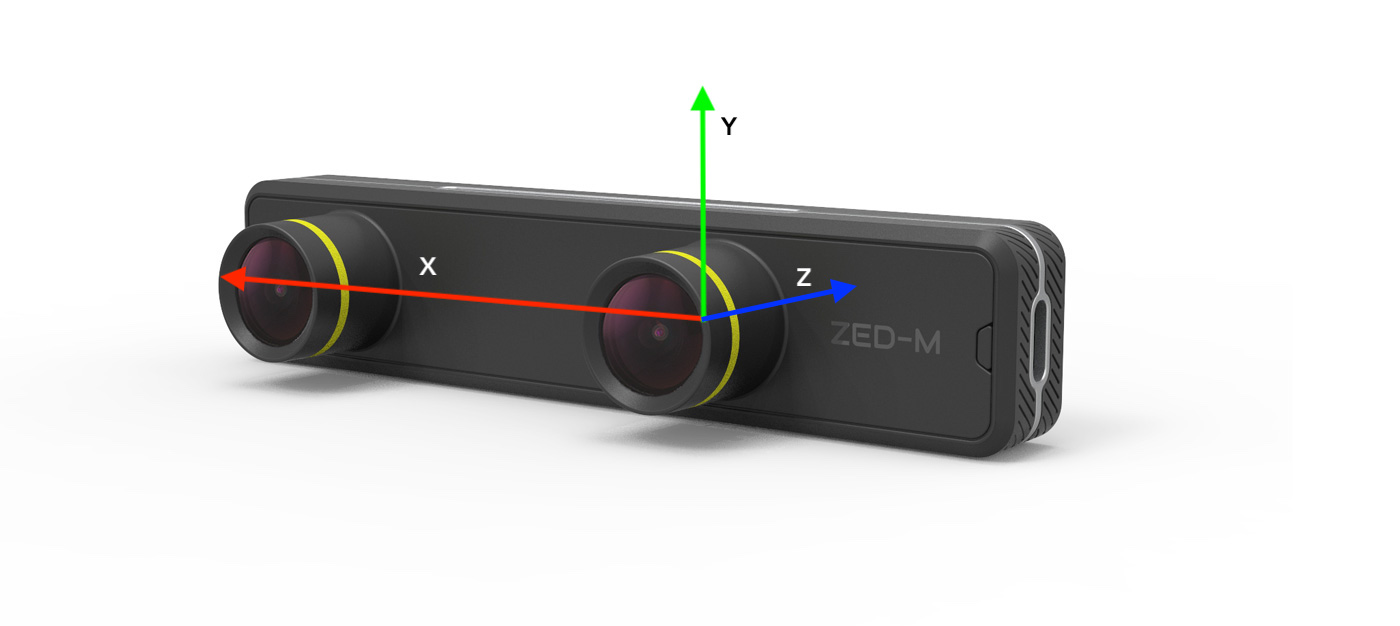
\includegraphics[width=0.9\linewidth]{images/zed_mini_coordinate_frame.jpg}
    \caption{ZED Mini coordinate frame (right-handed y-up)}
    \label{fig:zed_mini_coordinate_frame}
\end{figure}
% Add frame of reference

These points must be scaled to place them on the occupancy grid. This occupancy grid
extends \SI{15}{\metre} in front of the wheelchair and \SI{5}{\metre} on either side,
with each cell of the grid corresponding to a $\SI{25}{\milli\metre}\times \SI{25}{\milli\metre}$ area.
\Cref{eq:occupancy_scaling} was used to scale these points. Note that $p_x$ and $p_z$ are
represented in metres.
\begin{align}
i_x = max\left(min\left(\frac{p_x + 5.0}{0.025}, 1\right), \frac{10.0}{0.025}\right) - 1\\
i_y = max\left(min\left(\frac{p_z + 15.0}{0.025}, 1\right), \frac{15.0}{0.025}\right) - 1
\label{eq:occupancy_scaling}
\end{align}

% add before and after morphology as well as segmented image
Figure X shows the 2D occupancy grid after these steps have been completed,
with the drivable area labelled in green and the wheelchair represented in blue.
An issue with this occupancy grid is that it is rather sparse. The one-to-one
mapping between segmented pixels and grid cells causes the occupancy grid
drivable area to be discontinuous. To fix this, morphological dilation
was used ($10\times 10$ kernel) to improve the density of the occupancy map.
The result of this morphological processing can be seen in Figure X.

Although this approach reliably maps drivable areas to an occupancy grid,
the area directly in front of the wheelchair is unknown due to the FOV of the camera.
Some potential approaches to fix this are mentioned in the future work section of this thesis.
% still need to add speed

\subsection{Identification of static obstacles using 3D point cloud data}
% sensor tilt, find_floor_plane
% compare performance vs ultra depth mode
Another method to identify environmental obstacles and drivable areas
is direct processing of the 3D point cloud data, removing any use of the original RGB image data.
One such approach that was tested was the inbuilt ZED SDK function \texttt{find_floor_plane},
which identifies the floor plane and returns a 3D polygon of the floor plane location.
To display this floor plane, the polygon was projected onto the 2D XZ plane and displayed
using the python Pillow library. Results from this approach were very poor,
as seen in Figure X.

\subsection{Evaluation of semi-autonomous assistive wheelchair control algorithm}
% VFH+

\subsection{Comparison and implementation of wheelchair movement tracking algorithms}
% positional tracking API
